% chapters/searching.tex

\chapter{Searching}	\label{chapter:searching}

% deterministic search
Algorithm \ref{alg:deterministic-search} (see Problem $5-2$ of \cite{CLRS09})
searches for a value $x$ in an unsorted array $A$ consisting of $n$ elements 
by checking $A[1], A[2], \cdots, A[n]$ in order until either it finds $A[i] = x$
or it reaches the end of the array.

% file: algs/deterministic-search.tex

\begin{algorithm}[H]
  \caption{Deterministic search.}
  \label{alg:deterministic-search}
  \begin{algorithmic}[1]
    \Procedure{Deterministic-Search}{$A[1 \cdots n], x$}
      \State $i \gets 1$

      \hStatex
      \While{$i \le n$}
	\If{$A[i] = x$}
	  \State \Return $true$
	\EndIf
	\State $i \gets i + 1$
      \EndWhile

      \hStatex
      \State \Return $false$
    \EndProcedure
  \end{algorithmic}
\end{algorithm}

% binary stride
\begin{figure}
  \centering
  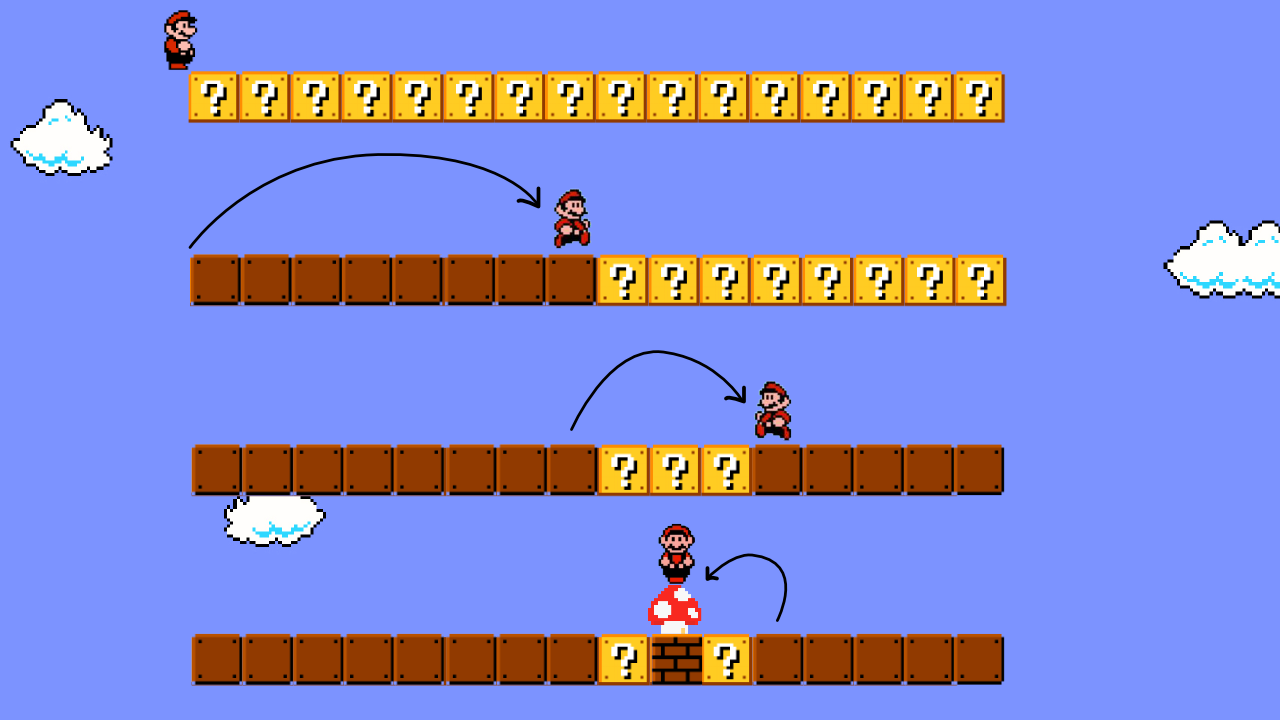
\includegraphics[width = 0.70\textwidth]{figs/binary-stride}
  \caption{Binary stride.}
  \label{fig:binary-stride}
\end{figure}

% file: algs/binary-search-iterative.tex

\begin{algorithm}[H]
  \caption{Iterative binary search.}
  \begin{algorithmic}[1]
    \Procedure{BinarySearch}{$A[0 \cdots n-1], x$}
      \State $L \gets 0$
      \State $R \gets n-1$

      \hStatex
      \While{$L \le R$}
        \State $m \gets L + (R - L) / 2$

	\hStatex
	\If{$A[m] < x$}
	  \State $L \gets m + 1$
	\ElsIf{$A[m] > x$}
	  \State $R \gets m - 1$
	\Else
	  \State \Return $m$
	\EndIf
      \EndWhile

      \State \Return $-1$
    \EndProcedure
  \end{algorithmic}
\end{algorithm}


% file: algs/binary-search-recursive.tex

\begin{algorithm}[H]
  \caption{Recursive binary search.}
  \begin{algorithmic}[1]
    \Procedure{BinarySearch}{$A, L, R, x$}
      \If{$R < L$}
	\State \Return $-1$
      \EndIf

      \hStatex
      \State $m \gets L + (R - L) / 2$

      \hStatex
      \If{$A[m] = x$}
	\State \Return $m$
      \ElsIf{$A[m] > x$}
	\State \Return $\Call{BinarySearch}{A, L, m-1, x}$
      \Else
	\State \Return $\Call{BinarySearch}{A, m+1, R, x}$
      \EndIf
    \EndProcedure
  \end{algorithmic}
\end{algorithm}

